\documentclass[11pt, a4paper, oneside]{article} % article scrartcl
\usepackage[utf8x]{inputenc}		% Umlaute können genutzt werden ohne \" davor zu stellen
\usepackage{ucs}					% contains support for using UTF-8 as input encoding
\usepackage{amsmath}				% besser Mathe-Ausgabe
\usepackage{amsfonts}				% Mathe-Schrift
\usepackage{amssymb}				% Mathe-Symbole
\usepackage[ngerman]{babel}			% für deutsche Sprache. Übersetzungen (z.Bsp. Zusammenfassung <-- Abstract) und Silbentrennung 
\usepackage{fancyhdr}				% für Kopf- und Fußzeilen
\usepackage{graphicx}				% für Bilder
\usepackage{graphics}				% für Bilder
\usepackage{url}					% für anklickbare URLs
\usepackage{parskip}				% kein Einrücken sondern Leerzeilen zwischen Abschnitten
\usepackage{color}					% Farben
\usepackage{units}   				% Einheiten, \unit[23]{m}
\usepackage{hyperref}				% Referenzen
\usepackage{todonotes}				% Todo
\usepackage{listings}

\author{Martin Junghanns \\  \url{martin.junghanns@studserv.uni-leipzig.de} \and 
		Sascha Ludwig \\ \url{s.ludwig@studserv.uni-leipzig.de} \and 
		Robert Schulze \\ \url{robert.schulze@studserv.uni-leipzig.de} }
\date{\today}
\title{ Performanz Evaluation von Graphdatenbanksystemen versus MySQL am Beispiel von Kookkurrenzgraphen }

% Standardpfad fuer Grafiken
\graphicspath{
 {./pics/}
}

\begin{document}

% bei Aufzählungen einen Strich an Stelle eines Punktes verwenden
\renewcommand{\labelitemi}{-}

% Titel mit Autoren
\maketitle

% Abstract
\begin{abstract}
	Dieser Bericht ist die Zusammenfassung der Praktikumsergebnisse im Rahmen des Moduls \dq Fortgeschrittene Methoden des Information Retrieval\dq~im WS 2010/11 der Universität Leipzig. Inhalt des Praktikums war die Evaluation verschiedener Graphdatenbanken und die Gegenüberstellung von relationalen Datenbanken. Als Vertreter der Graphdatenbanken wurden Neo4j, DEX und OrientDB näher betrachtet, MySQL wurde als relationale Datenbank in den Vergleich einbezogen.\\
Konkrete Ziele des Praktikums waren das Kennenlernen der verschiedenen Graphdatenbanken, der zu Grunde liegenden Datenmodelle und deren Abfragetechniken. Für den experimentellen Vergleich sollten verschiedene Kookkurrenzgraphen des Wortschatz Leipzig Projektes in die jeweilige Datenbanken importiert und mit den individuell angebotenen Möglichkeiten abgefragt werden. Dabei wurden ausgewählte SQL-Anfragen in API-Anfragen, aber auch in deklarative Anfragesprachen des jeweiligen Herstellers umformuliert und hinsichtlich ihrer Ausführungszeit verglichen.\\
Um die gemessenen Ausführungszeiten besser vergleichen zu können wurden die Messergebnisse mittels genuplot\footnote{\url{http://http://www.gnuplot.info/}} visualisiert.
\end{abstract}

\listoftodos

\section{Projektbeschreibung}
	Als Ergebnis des Praktikums ergaben sich zum einen konkrete und vergleichbare Messergebnisse der einzelnen Datenbanken. Zum anderen ist ein minimales, einfach konfigurierbares und auf den Anwendungsfall des Datenbankenvergleichens angepasstes Benchmarkframework entstanden. Das Framework unterstütze uns beim aggregieren der Messergebnisse einzelner Datenbanken und erleichterte wiederkehrende Aufgaben. 
	
\subsection{Softwarearchitektur}
Das Framework besteht aus sechs Komponenten, durch deren Ableitung und Kombination sich ein einzelner Benchmarkvorgang durchführen lässt, die im folgenden kurz vorgestellt werden sollen. 

\subsubsection{Konnektoren}
Ein Konnektor (Connector) dient den einzelnen Benchmarks oder Importierern zur Herstellung und Aufrechterhaltung einer Verbindung zur jeweiligen Datenbank. Für jede Datenbank muss nur ein Konnektor implementiert werden.

\subsubsection{Importierer}
Ein Importierer (Importer) dient dem Importiervorgang einer Datenbasis in die jeweilige Datenbank. In unserem Fall wurde die Datenbasis aus einer MySQL Datenbank übernommen. An dieser Stelle könnte aber auch ein Import aus einer CSV-Datei oder mit einer anderen Quelle implementiert werden. Für den vorstellbaren Fall, dass Benchmarks nicht auf einer existierenden Datenbasis operieren, ist die Implementierung eines Importierers nicht notwendig. Durch den Importierer lässt sich eine Datenbank auch in den Urzustand zurücksetzen und alle enthaltenen Daten entfernen.

\subsubsection{Benchmark-Suite}
Eine Benchmark-Suite dient der Zusammenfassung mehrerer einzelner Benchmark zu einer Folge, die geordnet durchgeführt werden sollen. Die Benchmark-Suite ermöglicht das Aggregieren und Persistieren einzelner Messergebnisse. In der Benchmark-Suite kann konfiguriert werden ob der eigentlichen Messung vorausgehend eine sogenannte Aufwärmung der Datenbank durchgeführt werden soll oder nicht.

\subsubsection{Benchmark}
Ein Benchmark misst die durchschnittliche Ausführungszeit einer Datenbankoperation. Die auszuführende Datenbankoperation ist an dieser Stelle zu implementieren.

\subsubsection{Konfigurationsdateien}
Bezüglich geeigneter Parameter ist die Konfiguration der einzelnen Datenbanken oder des Frameworks selbst über sogenannte properties-Dateien möglich.

\subsubsection{Auswärtungsskripte}

\subsection{Bedienungsanleitung}
\label{subsec:bedienungsanleitung}

\subsubsection{Vorraussetzungen}

\begin{itemize}
\item repository auschecken
\item maven dependencies installieren
\item etc.
\item pp.
\end{itemize}

\subsubsection{Benchmarks ausführen}


\subsubsection{Benchmarks konfigurieren}

\subsubsection{zusätzliche Benchmarks}

\subsubsection{zusätzliche Datenbank}

\subsection{Einschränkungen}

Vorhandene Einschränkungen Datenbank-spezifischer Natur sind im jeweiligen Abschnitt dokumentiert.

An dieser Stelle sei aber auch erwähnt, dass wir im Rahmen des Praktikums keine überdurchschnittliche Expertise bezüglich der verwendeten Datenbanken ausbilden konnten und so die Aussagekraft unserer Messergebnisse unter folgendem Bedingungen zu betrachten sind: Es ist durchaus möglich, dass sich die in den Benchmarks verwendeten Datenbankoperationen noch weiter optimieren ließen. Dabei kann es sein, dass eine Optimierung nur hinsichtlich bestimmter Operationen einen Vorteil bringt und sich bei andere Operationen eher nachteilig auswirkt.

\subsection{Erweiterungsmöglichkeiten}

Bezüglich der Erweiterungsmöglichkeiten muss an dieser Stelle unterschieden werden. Zum einen ist es möglich die Benchmarks an sich zu erweitern, dazu siehe die Bedienungsanleitung im Absatz \ref{subsec:bedienungsanleitung}. Zum anderen bietet das Framework an sich Potenzial für Erweiterungen.

\subsubsection*{Vereinfachte Konfiguration der Benchmark-Suiten}
Es ist vorstellbar, dass die Erstellung einer Benchmark-Suite, also das Zusammenführen einzelner Benchmarks zu einer geordneten Folge, nicht zwingend in Programmierleistung in einer Java-Klasse geschehen muss. Denkbar wäre, dass man dies lediglich in einer properties-Datei konfiguriert. Dies vereinfacht das Anpassen einer Benchmark-Suite und ist auch für Personen ohne Programmierkenntnisse zugänglich.

\subsubsection*{Visualisierung von Messergebnissen durch das Framework}
Momentan geschieht die Auswertung der Messergebnisse noch außerhalb des Frameworks. Dazu existiert ein zusätzliches python-Skript, welches die Messergebnisse aggregiert, aufbereitet und mittels gnuplot visuell zugänglich ausgibt. Dieses aggregieren, aufbereiten und Ansprechen von gnuplot ist auch in Java möglich und könnte in das Framework integriert werden.

% der wahre Inhalt
\section{Neo4j}

Neo4j\footnote{\url{http://www.neo4j.org}} ist eine eingebettete, persistente, transaktionale Graphdatenbank. Sie wird seit 2005 von der Firma Neo Technology, Inc. entwickelt, Version 1.0 erschien Anfang 2010. Die Datenbank wurde vollständig in Java geschrieben und steht quelloffen zur Verfügung.\footnote{\url{https://github.com/neo4j/community}}

\subsection{Anbindung}

Neo4j kann in zwei verschiedenen Szenarien betrieben werden: Die eingebettete Version wird direkt in eine Java Applikation integriert und bietet den performantesten Zugriff auf die Datenbank. Darüber hinaus implementiert Neo4j eine REST Schnittstelle, mit welcher auf die Datenbank via HTTP Requests zugegriffen werden kann. Die Anbindung erfolgt über verschiedene Clients, welche den Zugang aus unterschiedlichen Plattformen und Sprachen heraus ermöglichen.\\
Für die Leistungsmessung wurde die eingebettete Variante der Datenbank genutzt. Sie bietet neben dem Geschwindigkeitsvorteil auch das volle Spektrum an Zugriffsmöglichkeiten an.

\subsection{Anfragemöglichkeiten}

Neo4j bietet verschiedene Möglichkeiten an, den gespeicherten Graphen zu traversieren bzw. abzufragen. Neben der nativen Java API und der ebenfalls in Java entwickelten Traversal API steht seit Version 1.5 mit Cypher eine deklarative Abfragesprache zur Verfügung. Die Beispielanfragen auf den Kookkurrenzgraphen wurden in allen drei Anfragemöglichkeiten formuliert und können im Code Repository eingesehen werden.

\subsection{Einschränkungen}

Die wesentlichen Einschränkungen von Neo4j beziehen sich auf die Anfragesprache Cypher und die Java basierte Traversal API. Cypher befindet sich im Entwicklungsstatus und bietet momentan keine Query Optimierung an. Dies führte in der Testumgebung zu Ausnahmen infolge von Speicherüberläufen während der Ausführung. Das gleiche Problem trat auch bei der Verwendung der Traverser API auf. Beide Anfragemöglichkeiten wurden in die Messungen nicht einbezogen, befinden sich jedoch ebenfalls im Code Repository.

\subsection{Dokumentation}

Von den betrachteten Datenbanken weist Neo4j die umfangreichste und ausführlichste Dokumentation auf, in konkreten Beispielen wird der Umgang mit der Datenbank erläutert. Die Javadoc wird automatisch mit jedem Release aktualisiert und jede Funktionalität ist ausreichend dokumentiert.\\
Darüber hinaus verwaltet Neo Technologies eine Mailing List auf der Probleme aktiv diskutiert werden. Neben der Verwendung der Datenbank werden innerhalb der Dokumentation auch Möglichkeiten der Optimierung aufgezeigt. Diese wurden im Rahmen des Praktikums in Anspruch genommen.

\subsection{Aussicht}

Neo4j befindet sich in einem aktiven Entwicklungsprozess. Anfragen an die Mailing List ergaben, dass insbesondere Cypher im Rahmen der nächsten Releases optimiert wird. Neo4j entwickelt außerdem mit Spring Data Neo4j eine Anbindung an das Spring Framework\footnote{\url{http://www.springsource.org/}}, welches die Integration in bestehende Softwaresysteme und die Abbildung zu Datenbankenobjekten stark vereinfacht.

\section{OrientDB}

OrientDB\footnote{\url{http://www.orientechnologies.com/}} ist eine eingebettete, persitente, transaktionale Dokumenten- und Graphdatenbank. OrientDB wird seit 1998 von Luca Garulli entwickelt. OrientDB ist zu 100\% in Jave implementiert und steht quelloffen zur Verfügung.\footnote{\url{http://code.google.com/p/orient/}}

\subsection{Anbindung}

OrientDB lässt sich innerhalb von Java Applikationen unkompliziert über eine Java API nutzen.\footnote{\url{http://code.google.com/p/orient/wiki/JavaAPI}} Neben einer Java-API bietet OrientDB auch die Möglichkeit der Steuerung des Datenbanksystems über eine eigene Konsole. Dies hat den Vorteil, dass man das Datenbanksystem erkunden und kennen lernen kann. In der Konsolen können Befehle in einer SQL-artigen Syntax\footnote{\url{http://code.google.com/p/orient/wiki/ConsoleCommands}} an das Datenbanksystem geschickt und ausgewertet werden.

\subsection{Anfragemöglichkeiten}
Auf die in OrientDB gespeicherten Daten kann im Großen und Ganzen auf drei verschiedene Arten zugegriffen werden. Die erste und performanteste Art ist der Zugriff mittels der nativen Java API. Diese kam auch in den Benchmarks zum Einsatz. \\
Weiterhin können Anfragen in einer SQL-artigen Syntax\footnote{\url{http://code.google.com/p/orient/wiki/SQL}} gestellt werden. Allerdings gibt es hier noch gewisse Einschränkungen laut des Autors "Sub-selects are not yet implemented." Dies hatte zur Folge, dass diese SQL-artige Art der Anfrage nicht für das in diesem Projekt beschriebene Problem genutzt werden kann. \\
Die Dritte Art der Zugriff kann mittels Gremlin\footnote{\url{https://github.com/tinkerpop/gremlin/wiki}} geschehen. Gremlin bietet eine an XPath angelehnte Syntax um Graphen zu traversieren.

\subsection{Einschränkungen}
Ein großes Bottleneck bei OrientDB ist der Import der Daten aus einer SQL-Datenbank. Auch nach dem Befolgen der "Performance Hints" und dem Optimieren diverser JVM Parameter, stieg die Zeit für den Import für die Kookurrenzen-Kanten exponentiell zur Anzahl der einzufügenden Kanten an (siehe Abbildung~\ref{fig:orientdb_import}). Dies hat zur Folge, dass große Datenmengen (ab 1M Datensatz mit 3349314 CO\_{}S Kanten) nicht mehr importiert werden konnten. Mittels JProfiler konnte der Persistierungsprozess von OrientDB als HotSpot ausgemacht werden. Ein Kontaktaufnahme mit dem Autor bezüglich dieses Performanzverlustes ist durch uns erfolgt, führte aber zu keiner Lösung des Problems.\\
Auch konnte die SQL-artige Abfragesprache OrientSQL nicht genutzt werden, da diese noch nicht alle Funktionalitäten von MySQL bereitstellt.

\subsection{Dokumentation}
OrientDB ist gut und ausführlich dokumentiert\footnote{\url{http://code.google.com/p/orient/wiki/Main}}, was das Arbeiten mit OrientDB einfach gestaltet. Es liegt sowohl eine komplette und ausführliche Javadoc der API\footnote{\url{http://www.orientechnologies.com/releases/latest/javadoc/index.html}} vor, als auch Informationsseiten zu grundlegenden und weiterführenden Aspekten vor. Auf diesen Webseiten lassen sich Informationen zu fast allen Fragen finden. Allerdings ist das Finden einer Antwort auf eine konkrete Frage teilweise schwierig. Dies ist unter Umständen dem Fakt geschuldet, dass OrientDB sowohl eine Dokumentendatenbank, als auch ein Key-Value-Store, als auch eine Graphdatenbank ist. Oft werden in der Dokumentation diese drei Konzepte vermischt, was zu Verwirrungen führen kann. Weiterhin hat das Fehlen eines ausführlichen und kompletten Einstiegbeispiels die Einarbeitung erschwert. Auch fehlen Beispiele für komplexe Anwendungsfälle. Allerdings war der Autor bei speziellen Fragen per E-Mail zu erreichen, wobei man auf eine Antwort lediglich eine angemessene Zeit warten musste.

\subsection{Aussicht}
OrientDB stellt bezüglich seiner Graphdatenbankenfunktionalität einige interssante Features in Aussicht. OrientDB stellt seit Kurzem eine Implementation der Tinkerpop Blueprints APIs zur Verfügung. Somit steht auch die einfache und leicht lesbare Highlevel-Abfragesprache Gremlin zur verfügbar. Mit dieser Abfragesprache ist es möglich auch komplexe und vielseitige Abfragen verständlich zu formulieren.

\section{DEX}

\section{Evaluation}

Im folgenden Abschnitt wird die Durchführung der Messung beschrieben. Dabei werden zunächst die verwendeten Anfragen vorgestellt und anschließend das Testbed beschrieben. Die Ergebnisse der Messung befinden sich im Anhang, eine Auswertung dieser ist in Abschnitt

\subsection{Anfragen}

Zur Messung wurden folgende Anfragen in den jeweiligen Sprachen bzw. APIs formuliert.

\subsubsection*{Anfrage 1}

Finde alle Satz- oder Nachbarschaftskookkurrenzen eines Wortes. Gib Frequenz, Signifikanz und die beteiligten Wörter der Kookkurrenz aus.

\subsubsection*{Anfrage 2}

Finde alle Satz- oder Nachbarschaftskookkurrenzen der Nachbarn eines Wortes. Gib Frequenz, Signifikanz und die beteiligten Wörter der Kookkurrenz aus.

\subsubsection*{Anfrage 3}

Finde alle Satz- oder Nachbarschaftskookkurrenzen zwischen den Nachbarn eines Wortes. Gib Frequenz, Signifikanz und die beteiligten Wörter der Kookkurrenz aus.

\subsection{Testbed}

Das Testsystem ist wie folgt aufgebaut: Intel Core i7 2620M (2 x 3,2Ghz), 8GB DDR3 RAM, Crucial M4 SSD Festplatte. Die Graphdatenbanken wurden in das Benchmark Framework eingebunden, MySQL wurde lokal installiert und mit den von MySQL vorgegebenen Einstellungen einer Produktivumgebung gestartet.\\
Die Auwahl der Knoten erfolgte zufällig, es wurde jedoch ein Seed Wert definiert um in jeder Datenbank die gleichen Startknoten zu verwenden. Darüber hinaus kann im Framework ein Schwellwert definiert werden. Dieser legt fest, wieviele ausgehende Kanten (Satz- oder Nachbarschaftskookkurrenz) ein zufällig ausgewählter Knoten mindestens besitzen muss. Dieser Wert wurde auf 20 festgelegt.
\par
Nachfolgend werden die Startparameter der Java Virtual Machine angegeben. Diese ergeben sich entweder aus der Dokumentation des Hersteller oder gewonnenen Erfahrungen infolge mehrere Testläufe.

\begin{lstlisting}
// MySQL
-server
-Xmx1g

// Neo4j
-Xmx4g
-server
-Xmn512M
-XX:+UseConcMarkSweepGC

// Dex
-server
-Xmx1g

// OrientDB
-server
-Xmx4g
-XX:+AggressiveOpts 
-XX:CompileThreshold=200
\end{lstlisting}


Hardware Fakten
Datensätze (Anzahl Knoten, Kanten, evtl. Gradverteilung)
cold caches / warm caches
JVM settings
versionen

\subsection{Auswertung}

\section{Fazit}



% Anhang auf neue Seite
\newpage
% und diese einspaltig
\onecolumn

\section{Anhang}

\begin{figure*}[htbp]
	\centering
	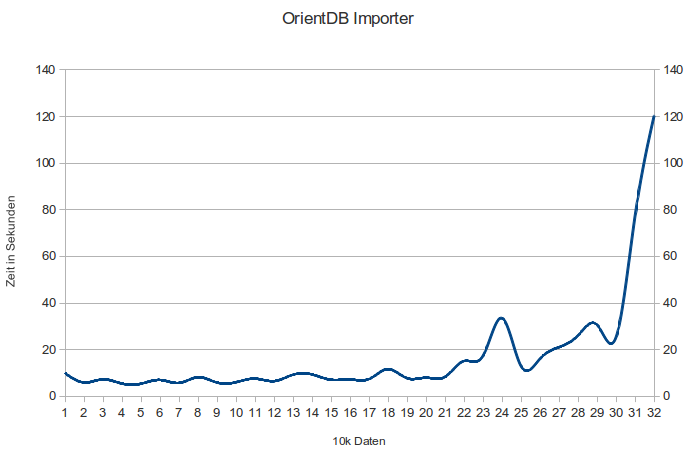
\includegraphics[width=10cm]{OrientImporter.png} 
	\caption{OrientDB-Importer Zeiten für Kookurenzen CO\_{}S}
	\label{fig:orientdb_import}
\end{figure*}


\end{document}